\section{Background}
\label{sec:background}

\IEEEPARstart{I}{n} this section, we will describe the OPM project and introduce the basic concepts used in the CFD field of reservoir simulation, such as grid, assembly, linear iteration, preconditioner, and linear solver. Also, concepts specific to reservoir simulation, such as the reservoir wells are defined.

\subsection{OPM Project}

Reservoir simulation\cite{reservoir_sim1,reservoir_sim2} uses mathematical models to predict the fluid flow dynamics in porous media. Typically, oil, water, and gas are modeled as fluids, and the porous media are usually rock or soil. The simulations can be used to improve reserve estimates, predict future production, or evaluate multiple reservoir management strategies. The first step is to create a static model of the reservoir, also called a geological model. This geological model is created by geologists and geophysicists by using multiple types of information, such as seismic data, well logs, production history, and rock properties. Important rock properties are type, porosity, water saturation, and permeability.

%%%%%%%%%% Flow summary
The Open Porous Media (OPM) \cite{OPM} simulator, OPM Flow \cite{flow_paper}, is an open-source simulator that models black-oil \cite{blackoil_model} with dissolved gas and vaporized oil. Other characteristics of the model that can be modelled include rock-dependent capillary and relative-permeability curves, end-point scaling and hysteresis, and oil vaporization controls. The simulator's input file is compatible with the commercial simulator Eclipse \cite{eclipse}, and the output file is readable by commercial post-processing software. The OPM project also features a post-processing software called ResInsight \cite{resinsight}. The black-oil model assumes three fluid phases (aqueous, oleic, and gaseous) and three components: water, oil, and gas. The oil and gas components represent all hydrocarbons in liquid and vapor form at standard conditions, respectively. Mixing is possible, so both oil and gas can be found in the oleic phase and gaseous phase. The partial differential equations (PDEs) are derived from the conservation of mass and Darcy's law\cite{darcy_law1,darcy_law2}, together with suitable initial and boundary conditions. The equations give each grid element three unknowns. Additionally, the wells each have equations and unknowns. Choosing which unknowns to solve for is important. For non-miscible flow, the oil pressure $p_o$, water saturation $s_w$, and gas saturation $s_g$ are chosen. For miscible flow, the gaseous phase may disappear if all the gas dissolves into the oleic phase. The oleic phase can also disappear if all the oil vaporizes into the gaseous phase. The oil pressure and water saturation are chosen, but the third variable is flexible:

\begin{equation}
    x = \begin{cases}
        s_g,      & \text{all three phases present,} \\
       r_{go},   & \text{no gaseous phase,} \\
      r_{og},  & \text{no oleic phase,} \\
    \end{cases}
\end{equation}

with $r_{go}$ being the ratio of dissolved gas to oil in the oleic phase, also called $r_S$ in other literature, $r_{og}$ being the ratio of vaporized oil to gas in the gaseous phase, also called $r_V$ in other literature.

The PDEs need to be discretized to be solved numerically. They are discretized in space with an upwind finite-volume scheme with a two-point flux approximation.
Discretization in time is done using an implicit backward Euler scheme. The derived equations form a system of fully implicit nonlinear equations. This system is solved using a Newton-Raphson method and linearized. The resulting linear system is solved with a preconditioner linear solver. Figure \ref{fig:flow_chart} shows the general structure of OPM Flow.

\begin{figure}[h]
\centering
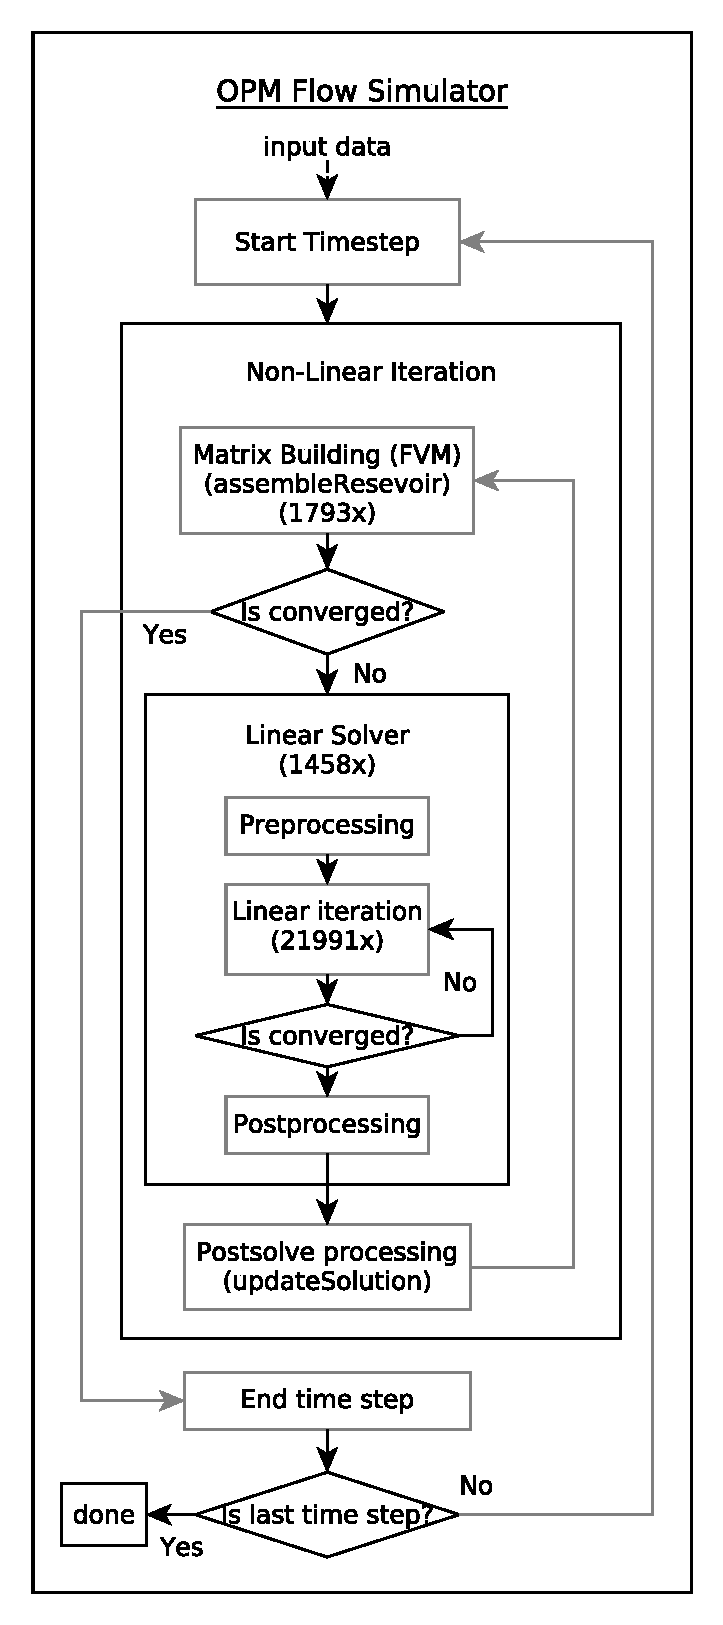
\includegraphics[scale=0.4]{figures/Flow_simulator_overview_CPU.pdf}
\caption{The General Structure of OPM Flow.}
\label{fig:flow_chart}
\end{figure}

%%%%%%%%%% grid
The reservoir is modeled by a grid, where each cell/element has its own properties, such as porosity, volume, or transmissibility. The grid properties are defined in input files, which include structure, faults, and various static rock properties like porosity and permeability. OPM supports 1D, 2D, and 3D models, with three types of grids: Cartesian Regular, Radial, and Irregular Corner-Point. The first two types are relatively simple but are also rather limited. Irregular Corner-Point grids are the industry standard for describing the structure of complex reservoirs. The Cartesian Regular grid defines a regular orthogonal grid. For Irregular Corner-Point grids, coordinates lines or pillars are given to indicate x and y coordinates. Then, the top and bottom surfaces are specified by the z-coordinates of the cell's corner points along the four adjacent pillars. The cell then forms an irregular hexahedron, with each cell having the same outline as the cell above or below when viewed from above. Radial grids can be used to model radial flow near a wellbore. The Radial grids in OPM are currently modeled as 2D cylindrical grids because no flow in the theta direction is implemented. Grids cannot be combined in OPM, so Irregular Corner-Point is mostly used. For more details on these grids, see the OPM Flow Reference Manual\cite{flow_manual}.

%%%%%%%%%% assembly
The simulation is fully implicit in time and has a flexible assembly of the linear system through automatic differentiation to enable rapid development of new fluid models. Traditionally, the closed-form expressions are obtained by differentiating the discretized flow equations by hand. This process is time-consuming and error-prone, but by using automatic differentiation, these drawbacks are removed. The simulator provides adaptive time step size controls. OPM Flow only uses Finite Volume Method (FVM), but the OPM project as a whole also implements Finite Element Method (FEM).%%%%%%%%%% linear solver
 The assembled linear system is blocked and sparse. The matrix is stored in the BCRSMatrix (block compressed row storage) datastructure, provided by dune-istl \cite{dune-istl}. Each block is a FieldMatrix, a dense matrix provided by dune-common. Due to fluid properties and other reservoir-specific parameters, the discretized equations could show elliptic, parabolic, or even hyperbolic behavior. The resulting linear system is usually non-symmetric and ill-conditioned.
Instead of solving the system directly, the solution is approximated by a preconditioned iterative solver. The solver can either be bicgstab (default) or restarted gmres. For preconditioner, the options are ILU0 (default), AMG, or CPR.

%%%%%%%%%% wells
OPM features two different well models: \textit{standard} and \textit{multi-segment}. A standard well has a single set of primary variables to describe the flow conditions inside. This works adequately for most wells and is, therefore, the default well model. For a three-phase black oil system, there are four primary variables: the weighted total flow rate, the weighted fractions of water and gas, and the bottom-hole pressure. %TODO: possibly elaborate the primary variables
 Each well object has three variables in the implementation that are used during the linear solve: B, C, and D. B and C are 1xNb blocked, sparse matrices, with MxN blocks, where Nb is the number of blockrows of the matrix, and M and N are 4 and 3 for blackoil respectively. D is a small MxM matrix. To apply a standard well, the solution vector x is a $C^T * (D^{-1} * (B * x))$. The multi-segment wells are used to simulate more advanced wells, such as multilateral wells, horizontal wells, and inflow control devices. The wellbore is divided into a number of segments, where each segment consists of a segment node and a flow path to the neighboring segment in the direction of the well head (outlet segment). Most segments also have inlet segment neighbors. Each segment has, in addition to the primary variables of a standard well, a node pressure variable.

%%%%%%
% OPM module structure
Finally, table \ref{tab:OPM_modules} lists the different OPM modules and their description.
\begin{table*}[!t]
\centering
\begin{tabular}{c|p{12.5cm}}
Name & Description \\ \hline
opm-common     & reads Eclipse data files, provides Python bindings, build systems \\
opm-grid       & provides interface for Dune-grid \\
opm-material   & deprecated, now inside opm-common, provided infrastructure to handle material properties like relative-permeability/capillary pressure, thermodynamic relations, and empirical heat conduction laws \\
opm-models     & contains fully-implicit numerical models for flow and transport in porous media \\
opm-simulators & contains simulator programs, like Flow, a fully implicit black-oil simulator that supports solvent and polymer options \\
\end{tabular}
\caption{Different OPM Modules and their Description.}
\label{tab:OPM_modules}
\end{table*}

%%%%%%
% ILU0 explanation
\subsection{ILU0}
To solve the linear system $Ax=b$ efficiently, the matrix $A$ is approximated by a factorization $A\approx LU$, with lower unitriangular matrix $L$ and upper triangular matrix $U$. Once we obtained such a LU factorization, solving the linear system is performed according to the equations (3) and (4), which is equivalent to solving (1), both methods leading to finding the unknown $x$ vector:

\begin{align}
    Ax &= b \\
    LUx &= b \\
    Ly &= b \\
    Ux &= y
\end{align}

The first equation (3) is solved using a forward substitution, and second, with the solution of $y$, a backward substitution is performed as in equation (4) to find $x$. The linear solves $Ly=b$ and $Ux=y$ are relatively easy since L and U are triangular matrices. In OPM terminology, this is called an ILU0 application, and the algorithm \ref{alg:ilu_apply} highlights this process.

% ILU decomp source:
% https://core.ac.uk/download/39699197.pdf

\begin{algorithm}
\caption{ILU0 application}
\label{alg:ilu_apply}
Input: vector x, vector b, matrix L, matrix U \\
Output: updated vector x 
\begin{algorithmic}
\STATE // forward substitution

\STATE // backward substitution
\end{algorithmic}
\end{algorithm}

For ILU0, L and U have the same sparsity pattern as matrix A. To find the $L$ and $U$ matrixes, a simple and sequential method to perform the decomposition is used, which is listed in Algorithm \ref{alg:ilu_decomp}.

\begin{algorithm}
\caption{ILU0 decomposition}
\label{alg:ilu_decomp}
Input: matrix A \\
Output: matrix A, but contains both L and U \\

// nb is the number of blockrows of A \\
\begin{algorithmic}
    

\STATE for r = 0 to nb: \\
    \STATE \hspace{0.5cm}d = 1/$a_{rr}$ \\
    \STATE \hspace{0.5cm}for i = r+1 to nb: \\
        \STATE \hspace{0.5cm} \hspace{0.5cm}if (i,r) exists in S: \\
        \STATE \hspace{0.5cm} \hspace{0.5cm}e = d*$a_{ir}$ \\
        \STATE \hspace{0.5cm} \hspace{0.5cm}$a_{ir}$ = e \\
        \STATE \hspace{0.5cm} \hspace{0.5cm}for j = r+1 to nb: \\
        \STATE \hspace{0.5cm} \hspace{0.5cm} \hspace{0.5cm}if (i,j) and (r,j) exist in S: \\
        \STATE \hspace{0.5cm} \hspace{0.5cm} \hspace{0.5cm} \hspace{0.5cm}$a_{ij}$ = $a_{ij}$ - e*$a_{rj}$ \\
\end{algorithmic}
\end{algorithm}


\subsection {GPU Architecture and Programming Model}
%%%%%%
% GPU computation
% small section on GPU architecture, CUDA vs OpenCL, AMD vs NVIDIA, warps, contiguous memory...
GPUs are traditionally designed for display purposes.
Since each pixel is independent of others, they can be processed in parallel.
This means the GPU has a parallel architecture.
It can also process other algorithms that have parallelism.

GPUs have a massively parallel architecture, which allows them to process large amounts of data in a relatively short time if the processing algorithm has enough parallelism.
The computation is done by stream processing.
Data can be read, processed, and written at the same time in a pipeline.
The two big manufacturers are NVIDIA and AMD.
NVIDIA proprietary language CUDA is only available for NVIDIA GPUs, and the open-source OpenCL can run on both.
For a kernel, a set of threads are launched, called workitems.
Workitems are organized in workgroups.
Workgroups can operate independently from each other, but the workitems in a workgroup are mapped to the same hardware area, a Streaming Multiprocessor (SM) on NVIDIA GPUs, or a Compute Unit (CU) on AMD GPUs.
The workitems are also divided into wavefronts of 64 workitems.
All 64 workitems execute the same instructions at the same time.
If the kernel contains a branch that is not taken by all 64 workitems, the branch is serialized.
Some of the workitems are deactivated, while the other take their branch; then activation is swapped, and the other branch is taken.
For NVIDIA GPUs, the wavefronts consist of 32 workitems.
Table \ref{tab:cuda_opencl_glossary} defines some of the OpenCL programming concepts and their CUDA counterparts.

It is important to only perform coalesced global memory accesses.
The workitems all perform the same global memory read/write instruction, but with slightly different addresses.
If the addresses are coalesced, the memory reads are combined into as many separate, serialized transactions as are needed.
If all workitems read from the same memory chunk, it only needs one transaction.

\begin{table}[h]
\centering
\begin{tabular}{c|c}
OpenCL & CUDA \\ \hline
wavefront & warp \\
workgroup & (thread)block \\
workitem & thread \\
local memory & shared memory \\
private memory & local memory \\
global memory & global memory \\
Compute Unit (CU) & Streaming Multiprocessor (SM)
\end{tabular}
\caption{Some OpenCL defintions and their CUDA counterparts.}
\label{tab:cuda_opencl_glossary}
\end{table}

